% !TeX root = ../main.tex
% Add the above to each chapter to make compiling the PDF easier in some editors.

\chapter{Einleitung}\label{chapter:introduction}

	%Calculating the integral of a function $f(x)$ is a typical problem in numerics. In many cases, the function $f(x)$ is not known but only the function values at certain, potentially arbitrary, points. In this scenario, a common approach is to approximate the integral using the finite set of sampling points. This is a non-trivial problem.
	
	%The term \term{term} is marked like this for better understanding.
	
	%\todo{This marks a todo}{}
	
	In den letzten Jahren gab es starke Entwicklungen auf dem Markt der sogenannten VR- und AR-Brillen \todo{VR anders benennen}. Dies kann man allein an der Menge neuer Geräte erkennen.
	Zwar gab es einen Rückgang der Verkaufszahlen in ...\todo{Verkaufszahlen rückgang zitieren}, die Prognosen für die kommenden Jahre sehen allerdings vielversprechend für diese Technologien aus.
	Neben bereits bekannteren Exemplaren wie der HTC Vive von den Firmen HTC und Valve, der Oculus Rift von Oculus VR oder der Hololens von Microsoft, gibt es nun auch billigere Umsetzungen wie die Daydream View von Google, welche das eigene Smartphone als Display verwendet. Zudem werden weiterhin verbesserte Versionen älterer Geräte veröffentlicht. Eins Beispiel dafür ist die HTC Vive Pro, welche sowohl in der virtuellen als auch, im Gegensatz zu ihrem Vorgängermodell, in der erweiterten Realität angewendet werden kann.\todo{Referenz}
	- Angebot für jedermann (durch verschiedene Preiskategorien)
	- es wird davon ausgegangen, dass Handy-VR durch seine geringe Leistungsfähigkeit in Zukunft wieder zurückgehen wird
	Und auch bei den Programmen für diese Brillen hat sich viel getan...
	- verschiedene VR Spiele und Anwendungen
	- auch crossplay, aber bisher fast ohne UI
	\todo{Fortsetzen!}

	\section{Was ist eine Benutzeroberfläche?}
		%- Schnittstelle zwischen Nutzer und Programm
		Im Bereich der Mensch-Maschine-Interaktion, kurz HCI (Human-Computer-Interaction) wird im Groben zwischen drei Bereichen unterschieden: Mensch, Maschine und deren Schnittstelle.\linebreak
		Die Benutzeroberfläche \todo{In Klammern: englisch user interface, UI} stellt eben jenen Übergang zwischen Maschine und Mensch dar und ermöglicht die Interaktion beider Seiten miteinander.\todo{Verweise!}
		%- nur die graphische Seite GUI betrachtet
		Sie lässt sich weiter in physische Steuerelemente und graphische Bestandteile (das GUI, engl. graphical user interface)\todo{Übersetzungen handhaben} aufteilen. Zu dem ersten Bereich zählen alle Arten von Knöpfen, Hebeln, Reglern und \todo{Fortsetzen}
		In dieser Arbeit wird allerdings nur der graphische Anteil betrachtet.
		
		%-Stellt Information zur Verfügung und ermöglicht die Erfassung und Manipulation der virtuellen Umgebung
		Er stellt dem Nutzer über Texte, Bilder und Farben Informationen zur Verfügung und kann deren Manipulation ermöglichen. Damit soll Benutzern die Erfassung und Veränderung der virtuellen Umgebung erleichtert werden.
		- Häufig als Menüs
	
		\subsection{Element}
			%- Beispiele: Textfeld, Bild, Schaltfläche...
			Die graphische Benutzeroberfläche setzt sich aus einzelnen Elementen zusammen. Diese können beispielsweise Texte, Bilder oder Schaltflächen sein, welche normalerweise innerhalb einer Menüstruktur untereinander oder nebeneinander angeordnet sind.
			\todo{Mehr! Anker erwähnen}
	
		\subsection{Anker}
			%- Position an welcher Elemente der Benutzeroberfläche platziert werden
			Ein Anker bezeichnet eine Position, zu welcher die Elemente der Benutzeroberfläche relativ platziert werden.
			\todo{Noch mehr dazu schreiben? Verweise suchen!}
			- In Desktop-Programmen werden dafür meist die Bildschirmkanten beziehungsweise Ecken verwendet
			%-Beispiel aus Unity
			\begin{figure}[htbp]
				\centering
				\includegraphics[width=0.4\textwidth]{figures/Ui_Anchor_Unity.png}
				\caption{Beispiel aus Unity that was taken from an external source \takenFrom{asc_notes}.}
				\label{fig:unity}
			\end{figure}
			\todo{Untertitel bearbeiten}
			
			An dem Beispiel aus der Spiel-Engine Unity (siehe \refFigure{fig:unity}), sieht man ... \todo{Weiter}
	
	\section{Was bedeutet umgebungsabhängig?}
		%- UI befindet sich im 3D Raum und kann von Objekten verdeckt werden. Sie ist an eine 3D Position gebunden und kann sich unabhängig vom Benutzer verschieben und rotieren, sie muss also nicht statisch zur Kamera sein
		Als umgebungsabhängig werden in dieser Arbeit Benutzeroberflächen bezeichnet, welche sich, im Gegensatz zum herkömmlichen zweidimensionalen Äquivalent, im dreidimensionalen Raum befinden und somit auch von Objekten aus der virtuellen oder realen Umgebung verdeckt werden können. Zudem müssen sie sich nicht statisch zu, beziehungsweise abhängig von, der Kamera bewegen, sondern können auch an einen anderen Gegenstand aus der Umgebung gebunden werden, mit dem sie sich mitbewegen und gegebenenfalls mitrotieren.
		- In 3D Programmen wird solche UI meist an Objekten positioniert und ist zu diesen statisch
		-In dieser Arbeit wurden als Ankerpunkte die beiden Handpositionen des Benutzers und die Kopfposition verwendet
	
	\section{Was ist VR/AR?}
		%- Augmented Reality = Erweiterte Realität
		%- Virtual Reality = Virtuelle oder künstliche Realität
		Die virtuelle Realität (VR) und die erweiterte Realität (AR, engl. augmented reality) \todo{Checken wie das gemacht wird} bilden zwei Teilbereiche der Vermischung von virtueller Welt und Realität, der sogenannten Mixed Reality (MR). So wird es jedenfalls in \todo{Zitiere Milgram} beschrieben. 
		
		\begin{figure}[htbp]
			\centering
			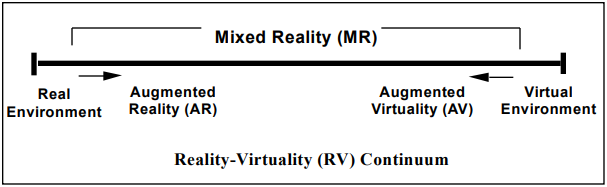
\includegraphics[width=0.75\textwidth]{figures/mixed_reality.png}
			\caption{Example picture that was taken from an external source \takenFrom{asc_notes}.}
			\label{fig:mixed_reality}
		\end{figure}
		\todo{Untertitel bearbeiten}
		
		- Head Mounted Display
		- Mischung von Realität und virtuellen Elementen
		- AR lebt von der realen Welt und somit von freiem Bewegen
		-> nicht an Pc gebunden
		--> weniger Leistung
		--> kein Handtracking